\documentclass{article}%
\usepackage[T1]{fontenc}%
\usepackage[utf8]{inputenc}%
\usepackage{lmodern}%
\usepackage{textcomp}%
\usepackage{lastpage}%
\usepackage{tikz}%
\usepackage{pgfplots}%
\pgfplotsset{compat=newest}%
%
\title{Continuous Integration}%
\author{MSO4SC}%
\date{\today}%
%
\begin{document}%
\normalsize%
\maketitle%
\section{2D 1 process}%
\label{sec:2D 1 process}%
\subsection{N Vertices {-} Convergence rate}%
\label{subsec:N Vertices {-} Convergence rate}%
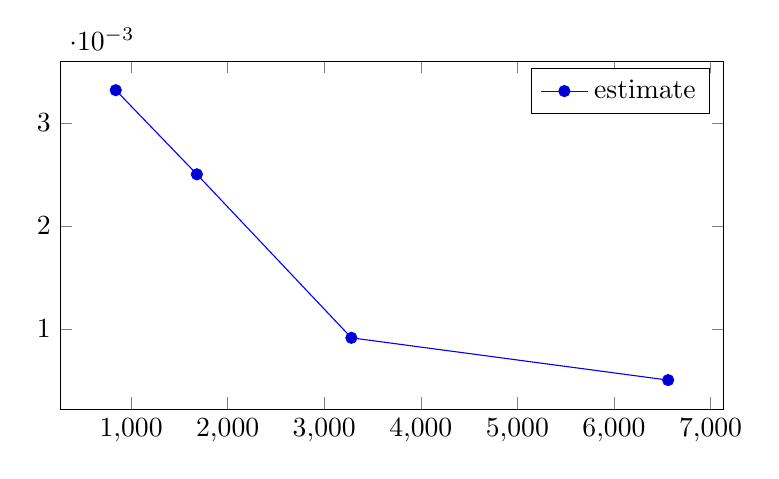
\begin{tikzpicture}%
\begin{axis}[height=6cm, width=10cm]%
\addplot coordinates {%
(841.0,0.00331676)%
(1681.0,0.0025003)%
(3281.0,0.000913458)%
(6561.0,0.000503076)%
};%
%
\addlegendentry{estimate}%
\end{axis}%
\end{tikzpicture}

%
\subsection{N Vertices {-} Errors}%
\label{subsec:N Vertices {-} Errors}%
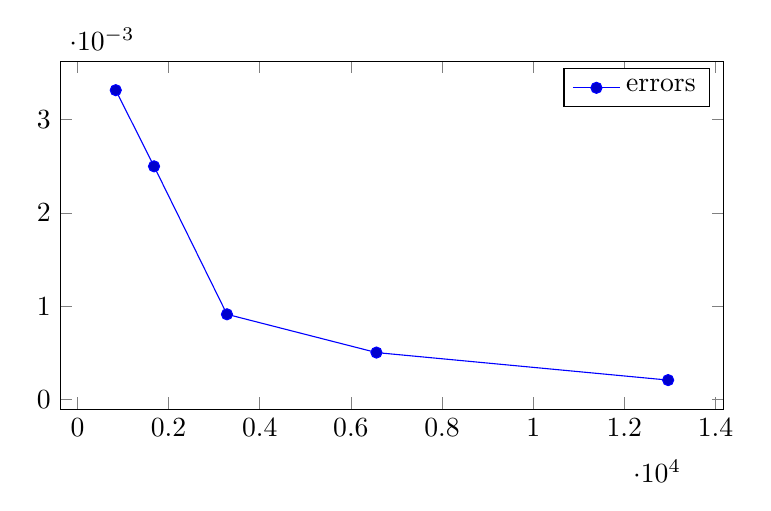
\begin{tikzpicture}%
\begin{axis}[height=6cm, width=10cm]%
\addplot coordinates {%
(841.0,0.00331676)%
(1681.0,0.0025003)%
(3281.0,0.000913458)%
(6561.0,0.000503076)%
(12961.0,0.000207921)%
};%
%
\addlegendentry{errors}%
\end{axis}%
\end{tikzpicture}

%
\subsection{N Vertices {-} Total time}%
\label{subsec:N Vertices {-} Total time}%
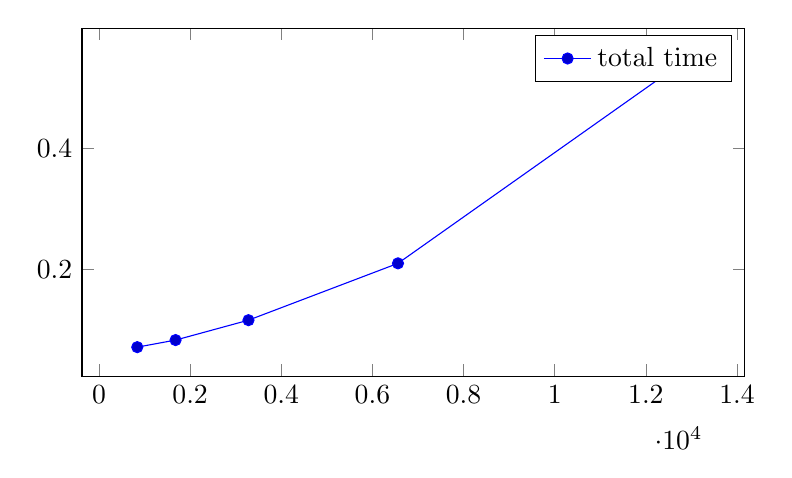
\begin{tikzpicture}%
\begin{axis}[height=6cm, width=10cm]%
\addplot coordinates {%
(841.0,0.072778)%
(1681.0,0.084414)%
(3281.0,0.117117)%
(6561.0,0.210529)%
(12961.0,0.54938)%
};%
%
\addlegendentry{total time}%
\end{axis}%
\end{tikzpicture}

%
\section{2D 5 process}%
\label{sec:2D 5 process}%
\subsection{N Vertices {-} Convergence rate}%
\label{subsec:N Vertices {-} Convergence rate}%
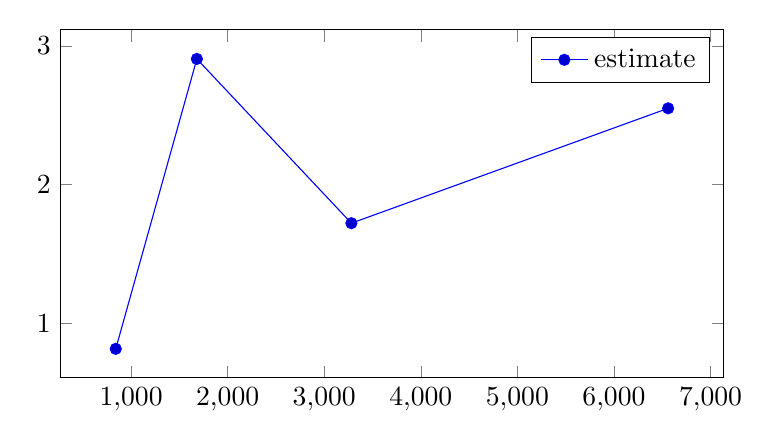
\begin{tikzpicture}%
\begin{axis}[height=6cm, width=10cm]%
\addplot coordinates {%
(841.0,0.815324268858)%
(1681.0,2.90546221004)%
(3281.0,1.7212111684)%
(6561.0,2.54934999992)%
};%
%
\addlegendentry{estimate}%
\end{axis}%
\end{tikzpicture}

%
\subsection{N Vertices {-} Errors}%
\label{subsec:N Vertices {-} Errors}%
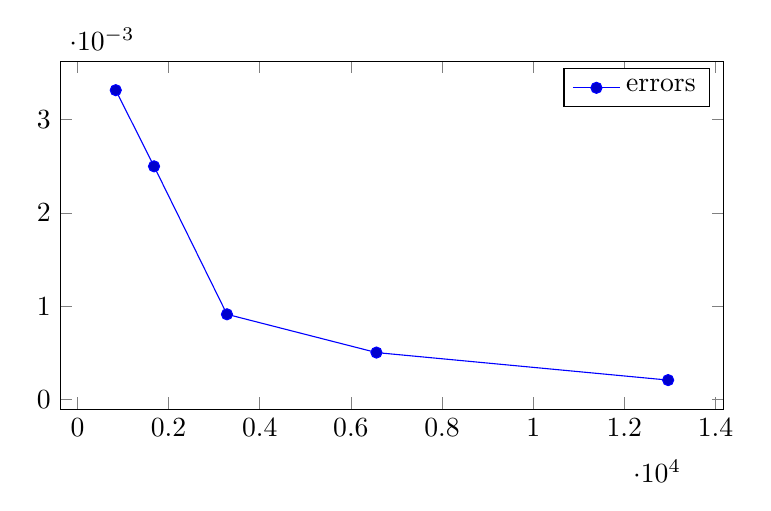
\begin{tikzpicture}%
\begin{axis}[height=6cm, width=10cm]%
\addplot coordinates {%
(841.0,0.00331676)%
(1681.0,0.0025003)%
(3281.0,0.000913458)%
(6561.0,0.000503077)%
(12961.0,0.000207921)%
};%
%
\addlegendentry{errors}%
\end{axis}%
\end{tikzpicture}

%
\subsection{N Vertices {-} Total time}%
\label{subsec:N Vertices {-} Total time}%
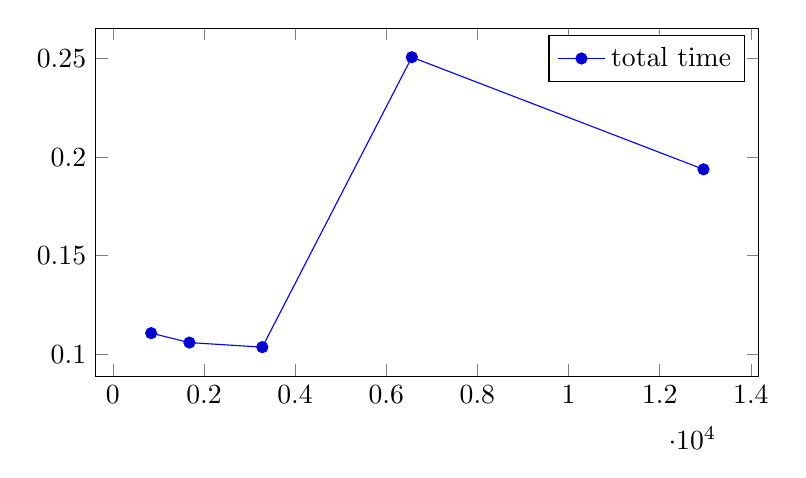
\begin{tikzpicture}%
\begin{axis}[height=6cm, width=10cm]%
\addplot coordinates {%
(841.0,0.110638)%
(1681.0,0.105854)%
(3281.0,0.10354)%
(6561.0,0.250744)%
(12961.0,0.193813)%
};%
%
\addlegendentry{total time}%
\end{axis}%
\end{tikzpicture}

%
\section{3D}%
\label{sec:3D}%
\subsection{N Processes {-} Strong Scaling}%
\label{subsec:N Processes {-} Strong Scaling}%
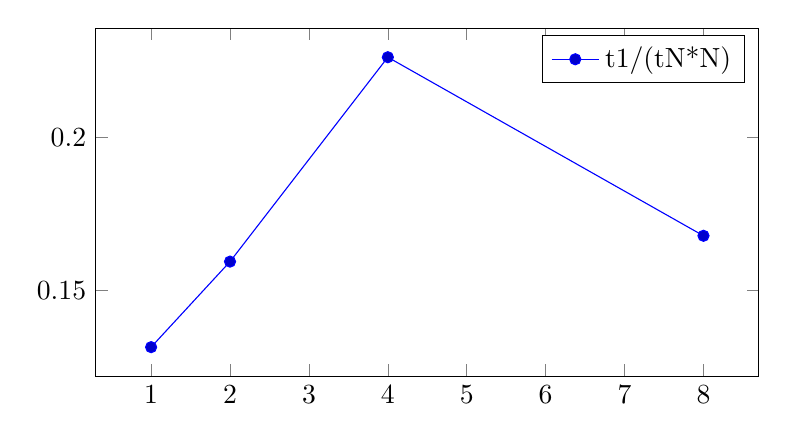
\begin{tikzpicture}%
\begin{axis}[height=6cm, width=10cm]%
\addplot coordinates {%
(1,0.131560584971)%
(2,0.159491374913)%
(4,0.22622561329)%
(8,0.167923459784)%
};%
%
\addlegendentry{t1/(tN*N)}%
\end{axis}%
\end{tikzpicture}

%
\subsection{N Processes {-} Weak Scaling}%
\label{subsec:N Processes {-} Weak Scaling}%
\begin{tikzpicture}%
\begin{axis}[height=6cm, width=10cm]%
\addplot coordinates {%
(1,1.0)%
(2,1.27177884341)%
(4,1.98230290575)%
(8,2.58299080893)%
};%
%
\addlegendentry{t1/tN}%
\end{axis}%
\end{tikzpicture}

%
\end{document}